\documentclass[a4]{article}
\usepackage[utf8]{inputenc}
\usepackage[french]{babel}
\usepackage{listings}
\usepackage{color}
\usepackage{graphicx}
\usepackage[T1]{fontenc}
\usepackage{pdfpages}
\usepackage{geometry}
\geometry{hmargin=2.5cm,vmargin=2.5cm}

\definecolor{mygreen}{rgb}{0,0.6,0}
\definecolor{mygray}{rgb}{0.5,0.5,0.5}
\definecolor{mymauve}{rgb}{0.58,0,0.82}

\lstset{
  backgroundcolor=\color{white},   % choose the background color; you must add \usepackage{color} or \usepackage{xcolor}
  basicstyle=\footnotesize,        % the size of the fonts that are used for the code
  breakatwhitespace=false,         % sets if automatic breaks should only happen at whitespace
  breaklines=true,                 % sets automatic line breaking
  captionpos=b,                    % sets the caption-position to bottom
  commentstyle=\color{mygreen},    % comment style
  deletekeywords={...},            % if you want to delete keywords from the given language
  escapeinside={\%*}{*)},          % if you want to add LaTeX within your code
  extendedchars=true,              % lets you use non-ASCII characters; for 8-bits encodings only, does not work with UTF-8
  frame=L,	                       % adds a frame around the code
  keepspaces=true,                 % keeps spaces in text, useful for keeping indentation of code (possibly needs columns=flexible)
  keywordstyle=\color{blue},       % keyword style
  language=C,                 	   % the language of the code
  otherkeywords={*,...},           % if you want to add more keywords to the set
  numbers=none,                    % where to put the line-numbers; possible values are (none, left, right)
  numbersep=5pt,                   % how far the line-numbers are from the code
  numberstyle=\tiny\color{mygray}, % the style that is used for the line-numbers
  rulecolor=\color{black},         % if not set, the frame-color may be changed on line-breaks within not-black text (e.g. comments (green here))
  showspaces=false,                % show spaces everywhere adding particular underscores; it overrides 'showstringspaces'
  showstringspaces=false,          % underline spaces within strings only
  showtabs=false,                  % show tabs within strings adding particular underscores
  stepnumber=2,                    % the step between two line-numbers. If it's 1, each line will be numbered
  stringstyle=\color{mymauve},     % string literal style
  tabsize=2,	                   % sets default tabsize to 2 spaces
  title=\lstname                   % show the filename of files included with \lstinputlisting; also try caption= instead of title
}
%gestion des caractères latins
\lstset{literate=
  {á}{{\'a}}1 {é}{{\'e}}1 {í}{{\'i}}1 {ó}{{\'o}}1 {ú}{{\'u}}1
  {Á}{{\'A}}1 {É}{{\'E}}1 {Í}{{\'I}}1 {Ó}{{\'O}}1 {Ú}{{\'U}}1
  {à}{{\`a}}1 {è}{{\`e}}1 {ì}{{\`i}}1 {ò}{{\`o}}1 {ù}{{\`u}}1
  {À}{{\`A}}1 {È}{{\'E}}1 {Ì}{{\`I}}1 {Ò}{{\`O}}1 {Ù}{{\`U}}1
  {ä}{{\"a}}1 {ë}{{\"e}}1 {ï}{{\"i}}1 {ö}{{\"o}}1 {ü}{{\"u}}1
  {Ä}{{\"A}}1 {Ë}{{\"E}}1 {Ï}{{\"I}}1 {Ö}{{\"O}}1 {Ü}{{\"U}}1
  {â}{{\^a}}1 {ê}{{\^e}}1 {î}{{\^i}}1 {ô}{{\^o}}1 {û}{{\^u}}1
  {Â}{{\^A}}1 {Ê}{{\^E}}1 {Î}{{\^I}}1 {Ô}{{\^O}}1 {Û}{{\^U}}1
  {œ}{{\oe}}1 {Œ}{{\OE}}1 {æ}{{\ae}}1 {Æ}{{\AE}}1 {ß}{{\ss}}1
  {ű}{{\H{u}}}1 {Ű}{{\H{U}}}1 {ő}{{\H{o}}}1 {Ő}{{\H{O}}}1
  {ç}{{\c c}}1 {Ç}{{\c C}}1 {ø}{{\o}}1 {å}{{\r a}}1 {Å}{{\r A}}1
  {€}{{\EUR}}1 {£}{{\pounds}}1
}
%definition d'un syle pour les documents texte
\lstdefinestyle{txt}{
	frame=none,
	numbers=none,
	stringstyle=\color{black},
}

\author{Alabi Steve - Benyamna Younes - Capdenat Nicolas- \\
		Chouipe Thibaut - El Harti Zakaria - Lienhardt Florian}
\title{Cahier Des Charges}
\date{\today}

\begin{document}
\maketitle
		\section{Preambule}
				Tout d'abord, nous allons parler de la steganographie, qui est "l'ancêtre" de la cryptographie. Elle se définit comme l'art de cacher un message dans un autre message. Cet "art"
				est appelé art de la dissimulation. Le mot steganographie vient du grec 	ancien 'steganós' qui veut dire "étanche" et 'graphein' qui signifie « écriture ». 		
				Exemples d'utilisation: 
				encre invisible sur une feuille, lettre de Georges Sand à Alfred Musset( la subtilité réside ici dans le fait qu'il faut lire une ligne sur deux de la lettre pour découvrir le vrai message)...etc
				Cependant, cet art présente une importante contre-mesure. En effet, si le message dissimulé est decouvert, le contenu secret esr revelé.

				Ainsi, un autre "art" s'impose: il est appelé art du secret et c'est justement la cryptographie. Ce dernier vient des mots en grec ancien 'kruptos', signifiant "caché" et 'graphein'
				signifiant lui "écrire". Globalement, cela consiste à protéger des messages. En effet, comme le dit Ronald Rivest, grand cryptologue américain et l'un des 3 inventeurs de l'algo
				de crypto à clé publique RSA, la crypto est la pratique et études des techniques pour assurer des communications sûres en présence d'adversaires.
				Trois critères doivent etre respectés : 
				-confidentialité : personne ne doit lire le message et on doit protéger le contenu.
				-authenticité : personne ne doit contrefaire l'origine du message et on doit s'assurer de la 							provenance de celui-ci.
				-intégrité : personne ne doit modifier le message et on doit s'assurer de la non-modification 							de celui-ci.

				La cryptographie, ainsi que la cryptanalyse(tout simplement l'art de rendre clair un texte crypté sans avoir connaissance de la clef utilisée) constituent la cryptologie.
				C'est un art ancien qui a commencé au 16eme siècle avant J-C par un potier qui avait gravé sa recette secrète en supprimant des consonnes et en modifiant l'orthographe des mots.
				C'est egalement une science nouvelle car elle est encore utilisée de nos jours dans plusieurs domaines tels que les banques(cartes), le web(navigateurs)..etc
				L'importance de la cryptologie se mesure par le fait qu'elle aie été utilisée lors des deux Guerres Mondiales. Selon certains spécialistes, les exploits des alliées en matière de cryptanalyse auraient même permis d'écourter la 2ème Guerre Mondiale d'un a deux ans.

				Après les guerres, une nouvelle forme de cryptographie liée a l'ère de l'informatique est apparue.
				
				Voici ci-dessous un tableau récapitulatif des différents chiffrements les plus connus :
				\\
				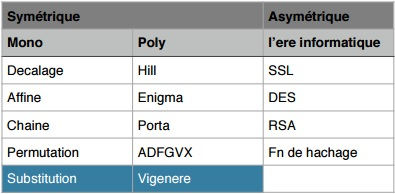
\includegraphics[scale=1]{Tab1.jpg}
				\\
				Nous allons lors de nôtre projet nous interesser aux deux suivants:\\
			Soit pour chaque lettre de l'alphabet son indice lui correspondant(a=0,b=1..z=25)			
			-Vigenère:
Le chiffrement de Vigenère consiste à faire une addition du texte en clair avec la clé(faire modulo 26).
Le dechiffrement lui se fait par soustraction du texte avec la clé ou à l'aide du test de Kasiski et de l'indice de coincidence si on ne connait pas la clé.
				-Substitution:
				Son chiffrement génère un nouvel alphabet: une lettre correspondra à une seule nouvelle lettre. Puis on utilise ce nouvel alphabet pour remplacer les lettres du texte clair.
				Le dechiffrement(avec connaissance de l'alphabet) consiste à effectuer l'operation précedente dans le sens inverse(chiffrement a->t,dechiffrement t->a). Sinon on effectue une analyse frequentielle afin de retrouver l'alphabet.
				
				
		\section{Fiches d'exigence}
				Vous trouverez les fiches d'exigences en annexe.
	\section{Numerotation des exigences}
				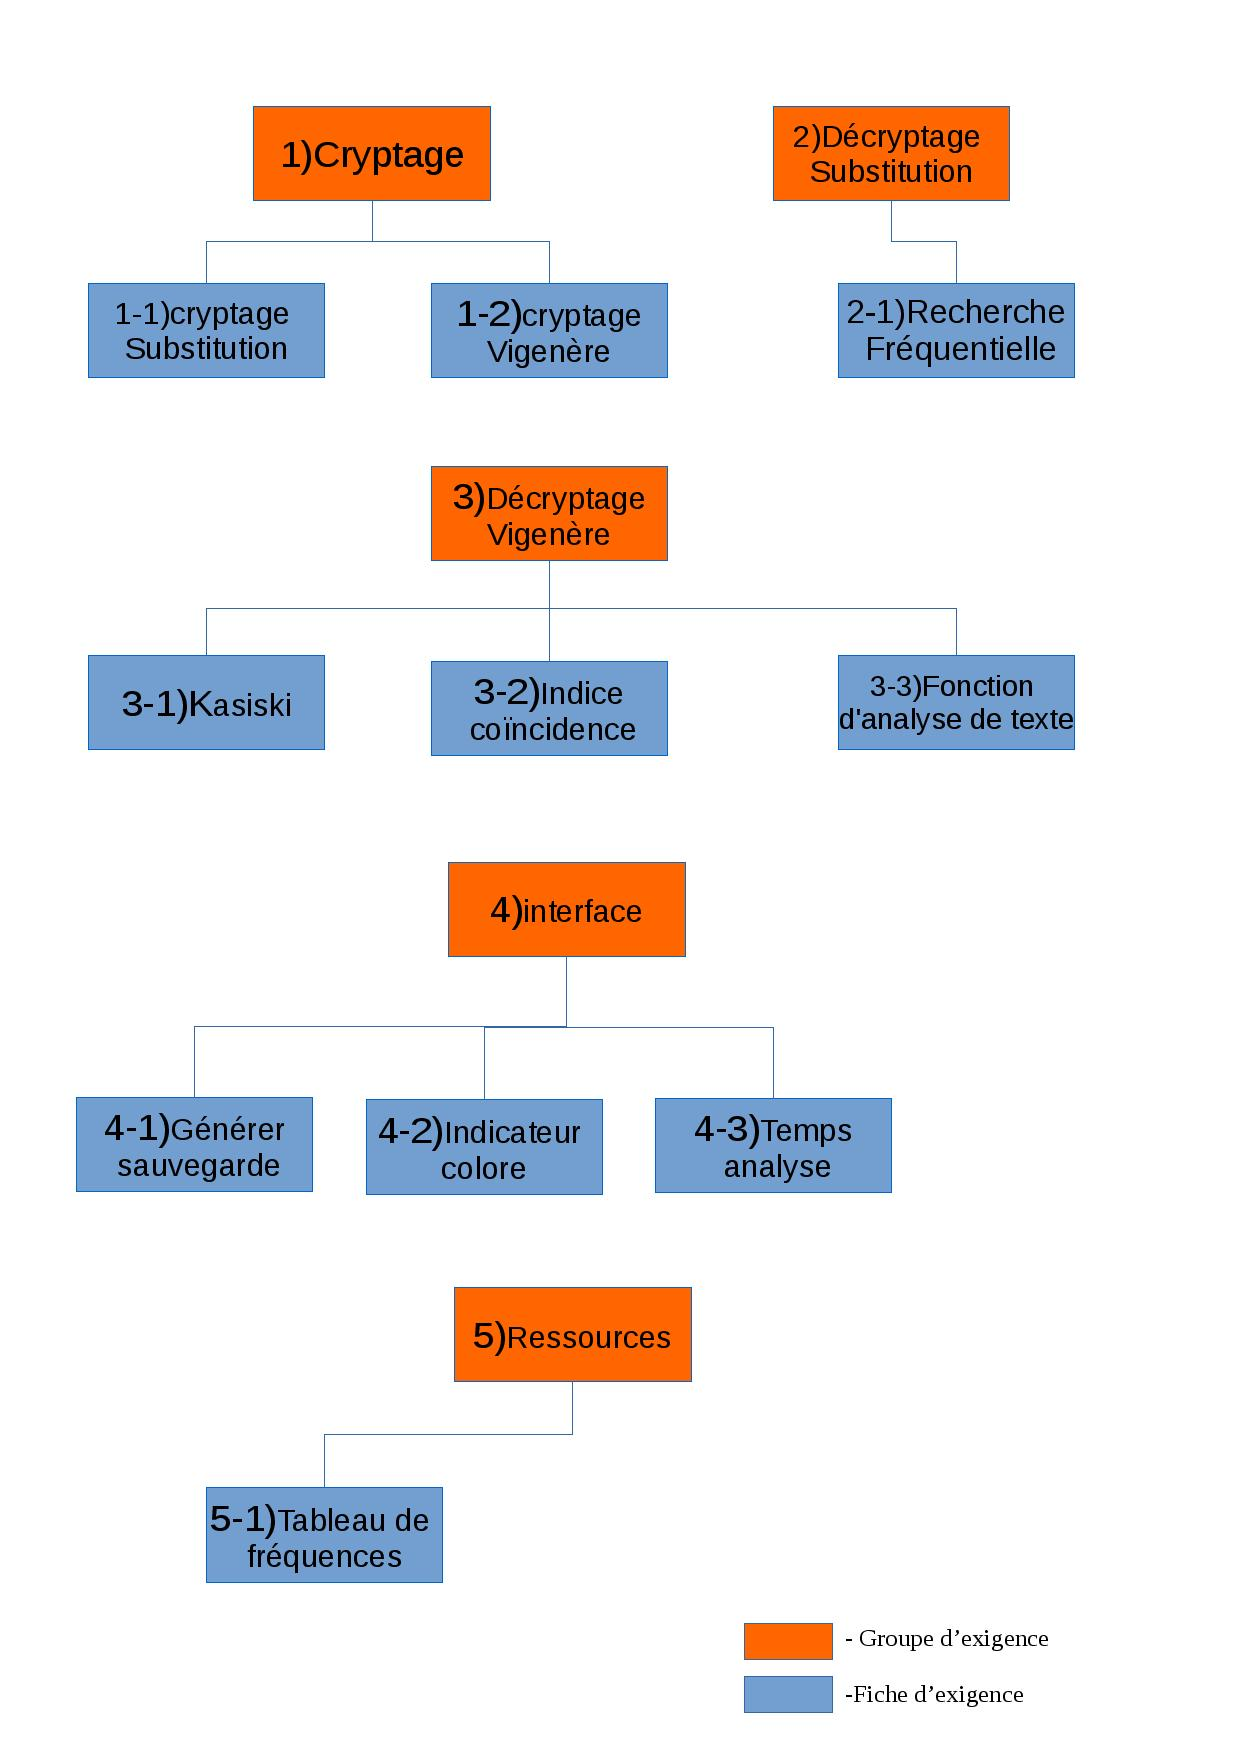
\includegraphics[scale=0.5]{Arbre.jpg} 
		
	\section{Fondement du projet}
		\subsection{But du projet} 
			\subsubsection{Problème de l'utilisation ou contexte du projet}
				Dans le cadre de notre L3, nous devons concevoir un programme d'aide au decryptage.
				Grace a notre programme le client(ici le professeur) va évaluer nôtre travail.
			\subsubsection{Objectif de la section}
				L'objectif de ce module est de nous apprendre a travailler efficacement en equipe afin de fournir un travail commun.
			\subsubsection{Objectif du projet}
				Le but du projet est de réaliser un logiciel automatique d'aide au décryptage, capable de retrouver une grande partie du texte d'origine à partir d'un texte chiffré. Il devra aussi être capable de déchiffrer le chiffrement de Vigenère et le chiffrement par substitution.
		\subsection{Personnes et organismes impliqués dans les enjeux du projet} 
			\subsubsection{Maitre d'ouvrage}
				Ce projet fait partie du module projet de la 3eme année d'informatique dirigé par Mme Kloul qui travaille au sein de l'UVSQ.			
		\subsection{Utilisateurs du produit}
			
	\section{Contraintes sur le projet}
		\subsection{Contraintes imposées non negociables} 
			\subsubsection{Contraintes sur la conception de la solution}
				-Le produit doit permettre à l'utilisateur de décrypter une partie d'un message crypté.

				-Le produit doit crypter ou décrypter un chiffrement de Vigenère et un chiffrement par substitution.

				-Toutes les deadlines concernant l'application et son cahier des charges doivent être respectées.
			\subsubsection{Environnement de fonctionnement du système actuel}
				Le produit sera développé sous forme d'application. 
				Le programme s'appuiera essentiellement sur des recherches fréquentielles pour décrypter un chiffrement par substitution et utiliser le test de Kasiski et les indices de coincidences pour déchiffrer par Vigenere.
			\subsubsection{Lieux de fonctionnement prévus}
				Il est préférable que l'utilisateur utilise un ordinateur moderne pour sa rapidité et sa fluidité.
			\subsubsection{ De combien de temps les développeurs disposent-ils pour le projet ?}
				La deadline pour les développeurs est le Vendredi 12 Juin 2017.
			\subsubsection{ Quel est le budget affecté au projet ?}
				Le client ne nous a pas référé son budget.
		\subsection{Glossaire et conventions de dénomination}
		
			k est la clé

			m est la taille de la clé

			n est la taille du message chiffré
			
			Les personnages Alice et Bob sont des figures classiques en cryptologie. Ces noms sont utilisés au lieu de « personne A » et « personne B » ; Alice et Bob cherchent dans la plupart des cas à communiquer de manière sécurisée.
			Alice est la personne qui envoie le message.
			Bob est celui qui veut recevoir le message.
			Oscar est celui qui essaye d'attaquer le message.
		\subsection{Faits et hypothèses utiles}	
			\subsubsection{Facteurs influençant le produit, mais qui ne sont pas des contraintes imposées sur les exigences}
	
		Mettre en place une interface facile d'utilisation sur l'application de manière a ce que même un enfant puisse lancer le décryptage.
	\section{EXIGENCES FONCTIONNELLES}
		\subsection{Portée du travail}
			\subsubsection{Situation actuelle}
				Nous n'avons aucune base pour notre application, nous allons la créer de toutes pièces.
			\subsubsection{Contenu du travail}
				Il est nécessaire de connaitre le chiffrement et le déchiffrement (avec et sans clé) de Vigenère et de substitution.
		\subsection{Portée du produit : cas d’utilisation}
			\subsubsection {Le diagramme de cas d'utilisation} 
				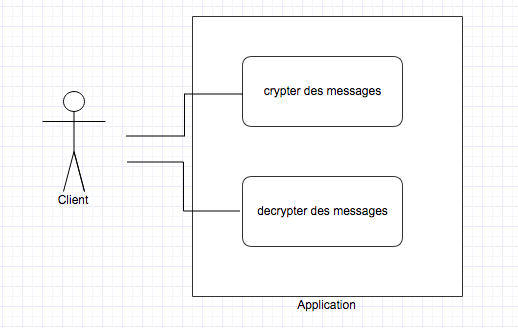
\includegraphics[scale=0.5]{dia.png} 
			\subsubsection {Description de ce diagramme}
				Dans cette application il n'y a qu'un seul type d'utilisateur qui est le client 
				et qui peut crypter et decrypter avec deux méthodes différentes à disposition.
		\subsection{Exigences fonctionnelles et exigences sur les données}
			\subsubsection {Exigences fonctionnelles}
				Fiches d'exigences numero : 2.1 / 3.1 / 3.2 / 3.3 / 5.1
	\section{EXIGENCES NON FONCTIONNELLES}
		\subsection{Ergonomie et convivialité du produit}
			\subsubsection {L'interface}
				L'interface permettra de rentrer facilement le texte à décrypter, par copier-coller par exemple.
				De plus, l'interface permettra de choisir la langue (anglais, français) grâce à un simple menu.
				Enfin, l'interface permettra aussi d'afficher facilement le resultat obtenu.
			\subsubsection {Le style du produit}
				Le programme sera évalué par la responsable du module Projet de la L3 donc il doit apparaître simple et effiace (pas de superflu).
				Le programme ne doit pas être trop gros en terme de resolution, on doit pouvoir l'afficher sur 	tous les types d'écrans d'ordinateurs.

		\subsection{Facilité d’utilisation et facteurs humains}
			\subsubsection {Facilité d'utilisation}
				Le programme sera simple à utiliser même pour un enfant.

				Le programme pourra etre utilisé par des personnes sans qu'elles y soient formées.
			\subsubsection {Personnalisation et internationalisation}
				Le programme sera trop simple pour etre personnalisable et il sera en anglais(simple a la compréhension).
			\subsubsection {Facilité d'apprentissage}
				Le developpement d'un site web présentant le produit ainsi que toutes ses caractéristiques. Ce site web pourra également disposer d'un forum permettant aux internautes de proposer certaines	améliorations à faire sur l'application et également critiquer certaines fonctionnalités de l'application.
				Il sera possible au grand public d’utiliser le programme sans formation.
			\subsubsection {Facilité de compréhension et politesse}
				Le produit devra utiliser des symboles et des mots naturellement compréhensibles par les
				utilisateurs potentiels.
				Le produit doit cacher les détails de sa construction à l’utilisateur.

		\subsection{Fonctionnement du produit}
			\subsubsection {Rapidité d’exécution et temps de latence}
				La réponse sera assez rapide pour éviter d’interrompre le flux de pensée de l’utilisateur.

			\subsubsection {Précision et exactitude}
				C'est un programme d'aide au décryptage donc il ne donnera jamais un texte complet en sortie 					mais un "texte à trou" rempli au mieux avec le résultat du décryptage.
			\subsubsection {Fiabilité et disponibilité}
				Le programme devrait être disponible pour une utilisation de 24 heures par jour et 365 jours
				par an. 

		\subsection{Adéquation du produit avec son environnement}
			\subsubsection {Environnement physique prévu}
				Le programme sera utilisé sur un ordinateur.
			\subsubsection {Environnement technologique prévu}
				Le programme pourra fonctionner sur Windows, Linux et Mac.
			\subsubsection {Approche « produit » prêt à être commercialisé}
					Le programme sera distribué sous forme d'archive correspondant au système 						d'exploitation du client.
		\subsection{Maintenance, support, portabilité, installation du produit}
			\subsubsection {Maintenance du produit}
				Le système doit pouvoir être maintenu par des développeurs qui ne sont pas les
				développeurs d’origine.
				Mettre en place une gestion des erreurs ou bugs (par exemple a l'aide de tests unitaire, 				d'indicateurs comme des variables..etc).
			\subsubsection {Conditions spéciales concernant la maintenance du produit}
				Site internet avec des informations sur l'application.
				Permettre également un dialogue avec d'autres utilisateurs de la même application.
				Demandes d'aide aux développeurs chargés de la maintenance de l'application.
			\subsubsection {Exigences en matière de support}
				L'utilisateur doit pouvoir communiquer avec d'autres utilisateurs et/ou les developpeurs en 					charge de la maintenance.
			\subsubsection {Exigences de portabilité}
				L'application peut fonctionner sur plusieurs environnements car "un makefile est fourni et 				permet a l'utilisateur de build en fonction de son environnement"(comme linux, windows ou autre).
			\subsubsection {Installation du système}
				L'application doit pouvoir être installée très facilement sur n'importe quel environnement.
				Le site internet doit permettre de répondre à certaines interrogations.
		\subsection{Sécurité}
			\subsubsection {Intégrité}
				Definition d'un niveau d'importance de "l'exactitude" nécessaire au dechiffrage du message.
				(exemple : les coordonnées pour envoyer un missile nucléaire doivent être ultras-précises)
			\subsubsection {Protection des données à caractère personnel}
				Message d'information a l'ouverture de l'application qui permet d'informer l'utilisateur des 					précautions à prendre.
			\subsubsection {Audit et traçabilité}
				Définition d'un repertoire de sauvegarde avec les dates des messages.
			\subsubsection {Protection contre les infections}
				Il faudra conserver les fichiers de maniere securisée et prudente ou alors les supprimer une 					fois que ce ceux-ci n'aient plus d'utilité.
		\subsection{Exigences culturelles et politiques}
			\subsubsection {Exigences culturelles}
				L'application pourra gérer plusieurs langues (plusieurs tableaux de frequences des lettres).
		\subsection{Lois et standards influençant le produit}
			\subsubsection {Conformité avec la loi}
				Les informations personnelles seront soumises a la loi sur la protection des données
				personnelles (Loi informatique et libertés).
			\subsubsection {Conformité avec des standards}
La notion de conventions de codage (coding style) désigne un ensemble de règles et de conseils 
adoptés par les membres d’un projet logiciel pour écrire et mettre en forme du code.
Les conventions de codage visent essentiellement à améliorer la lisibilité du code : elles doivent 
permettre au programmeur d’identifier « du premier coup d’œil » un maximum de choses dans 
le  code, de se repérer facilement, de savoir ou trouver les choses, etc.Une fois adoptés, elles
facilitent grandement l’écriture, la maintenance et aident à éviter certaines erreurs.
Dès lors qu’on travaille sur un projet logiciel d’une certaine ampleur, qui plus est à
plusieurs, l’expérience montre qu’il est très important de se mettre d’accord sur les
conventions de codage. Ainsi, nous avons décidé de définir nous même les règles a respecter durant le codage. Comme par exemple pour l'indentation, les noms des variables,les noms des fonctions..etc
\section{AUTRES ASPECTS DU PROJET}
		\subsection{Questions sans réponse}
		Nous pensons avoir abordé une grande partie des aspects du projet et des attentes du client.
		\subsection{COTS : progiciels et composants commerciaux}
		Il existe sur le marché pas mal de produits pouvant être des solutions potentielles/de remplacement. En effet, 			sur internet
		("en ligne"), il existe des sites proposant de decrypter votre texte. Nous avons par exemple testé le site 			www.dcode.fr, qui
		pour le dechiffrement avec Vigenere, fonctionne trés bien.
		Il y'a aussi une application (Decrypto) sur le Google Play Store (parmi plusieurs applis),qui est gratuite et 			qui permet aussi de dechiffrer Vigenere par exemple.
		Enfin, on peut telecharger des logiciels gratuits comme Axcrypt. Des logiciels payants/privés existent surement 			a l'usage des
		professionnels ou encore des services de police spécialisés.
		\subsection{Nouveaux problèmes, créés par le nouveau système}
		Il peut y avoir un problème de place ou mémoire lors de l'installation du "systeme" malgré que l'application 			soit légère.
		
		Un ralentissement de "l'environnement" peut aussi etre constaté a la suite de l'utilisation du nouveau 			système.
		\subsection{Tâches à faire pour livrer le système}
		Phase I: Identification du projet : La demande du client est clarifiée, les objectifs précisés et dans sa 			globalité le projet (ou service a livrer) est identifié. De plus, les contraintes a respecter sont 				evaluées et la strategie de realisation est mise en place.\\
		Phase II: Definition du projet : Son contenu est defini de maniere tres precise et la planification des 			echeances et de la repartition du travail est etablie.\\
		Phase III: Realisation : On realise le projet en adequation avec les exigences du clients et selon le plan de 			travail defini au prealable.\\
		Phase IV: Finalisation : Le produit est evalué puis remis au client.
		
		
		
		\subsection{Contrôle final de qualité sur site (Cutover)}
		Controle final sur un texte test. Un texte chiffré par vigenere et par substitution seront preparés, ainsi que 			leurs versions dechiffrées. Le resultat de ceux-ci via l'utilisation de l'application sera comparé a celui resultat 				preparé "sur feuille"(résultat théorique). 
		\subsection{Risques liés au projet}
		Avec l'utilisation de l'application, certains risques existent. En effet, une personne etrangère peut avoir 			accés a l'ordinateur et ainsi récupérer les fichiers decryptés telechargés ou les fichiers originals( avant cryptage).
		\subsection{Organigramme}
Détails des modules:\\ \\
		Interface graphique :\\
			- bouton cryptage\\
			- bouton decryptage\\
			- bouton substitution\\
			- bouton Vigenère\\
			- affichage de texte(complet et partiel)\\
			- affichage pour la clé de substitution\\
			- bouton Francais(decryptage)\\
			- bouton Anglais(decryptage)\\
			- affichage pour l'analyse fréquentielle\\
			- charger un fichier texte\\
			- sauvegarder un fichier texte\\
			- créer un nouveau fichier texte(resultats)\\
			- Demander clef de Vigenère\\
			
		Cryptage Substitution :\\
			- créer une clé aleatoirement\\
			- crypter le message\\
			
		Cryptage Vigenère :\\
			- crypter le message
			
		Decryptage Substitution :\\
			- decrypter le message\\
			
		Analyse fréquentielle :\\
			- analyse frequentielle sur texte donné\\
			
		Decryptage Vigenère :\\
			-decrypter le message
		
		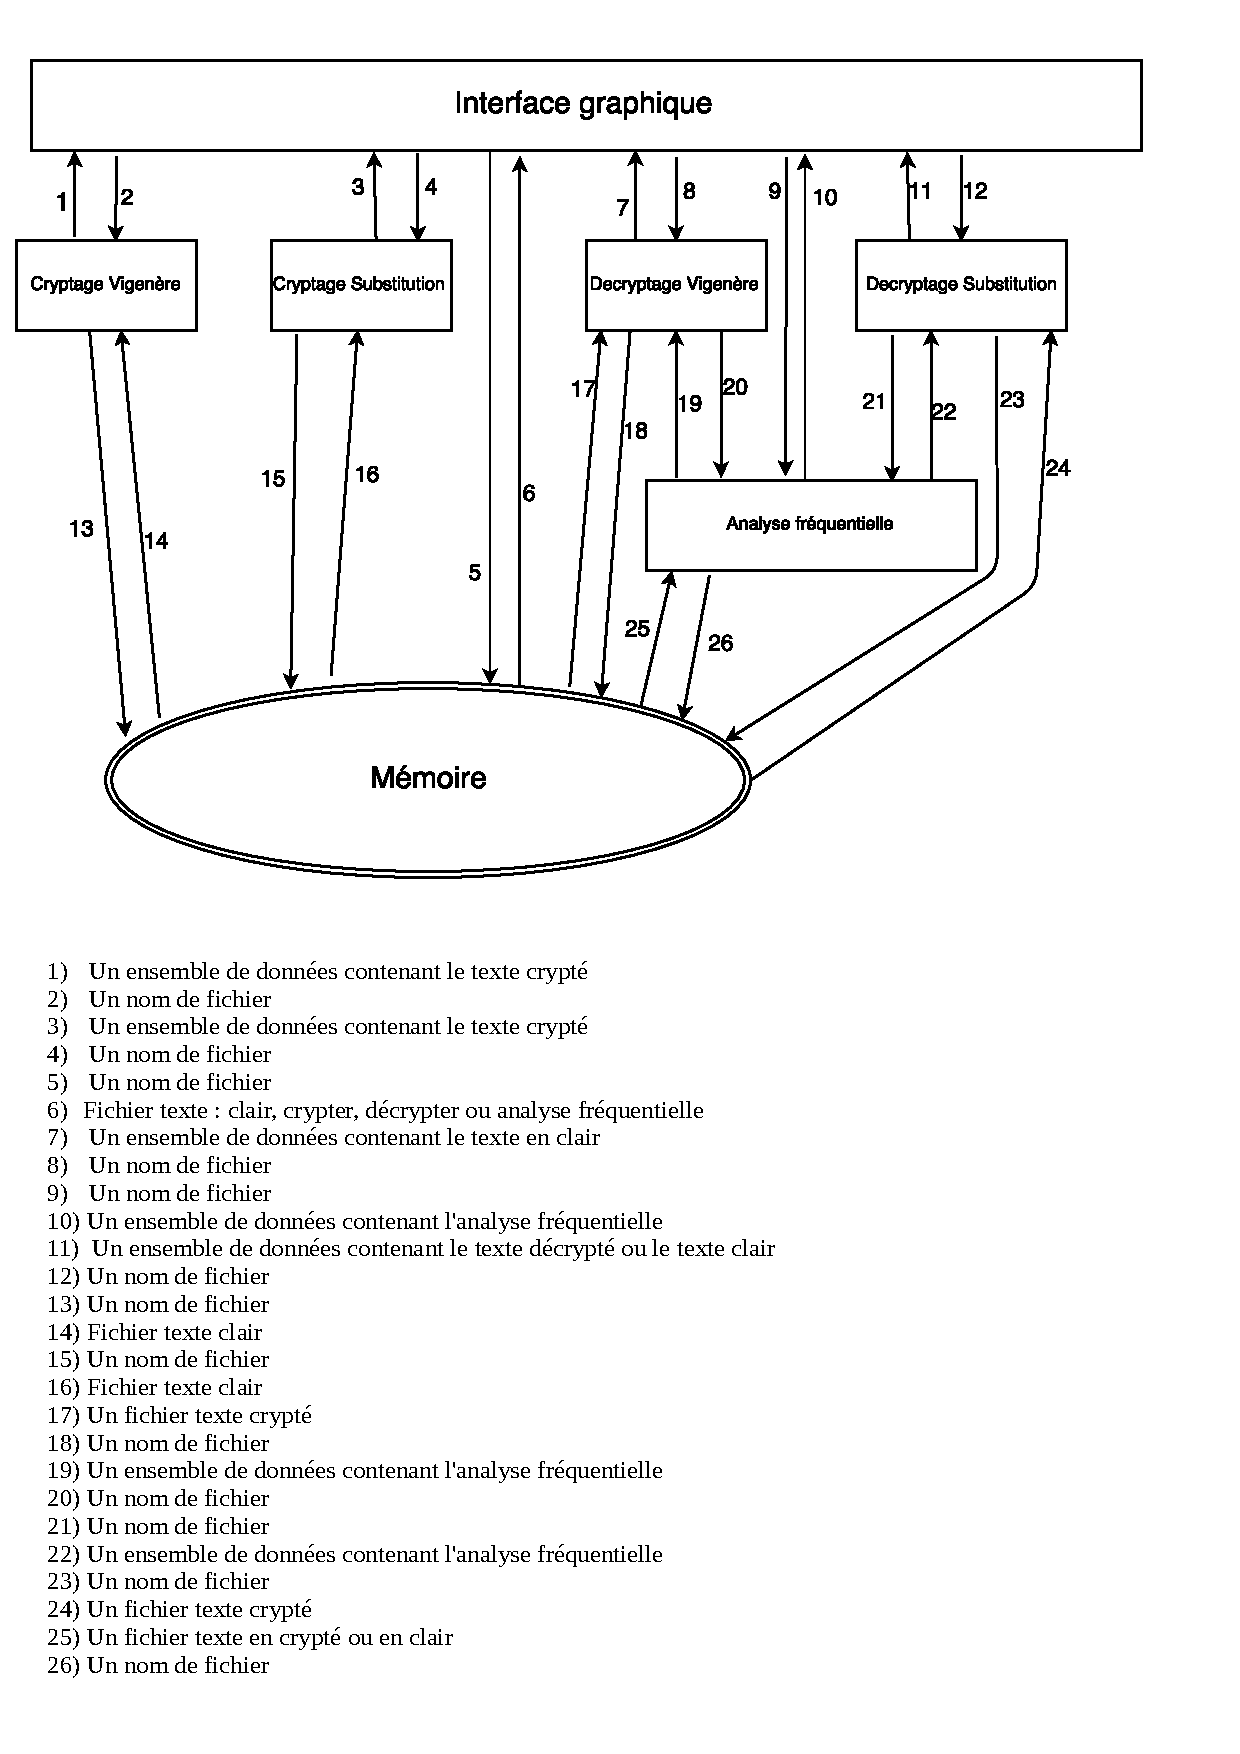
\includepdf[scale=0.7]{organigramme_final.pdf}


		\subsection{Estimation des coûts du projet}
		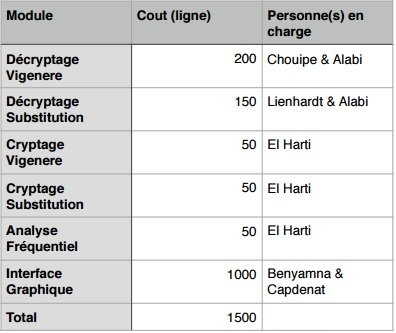
\includegraphics[scale=0.5]{Tableau_cout.jpg} 
		\subsection{Manuel utilisateur et formations à envisager}
			L'utilisateur aura accés à un menu lui permettant de choisir de crypter ou décrypter un texte,
			puis la méthode qu'il veut utiliser pour ce faire (vigenere ou substitution), il ne lui restera 
			plus qu'a importer son texte.
		\subsection{Salle d’attente : idées pour les futures versions}
			Bien que le programme ait été demandé que pour la langue francaise et anglaise, 
			il sera sans doute possible d'ajouter d'autres langues dans des versions futurs. 
			Il pourra être également possible d'ajouter une option permettant à l'utilisateur

			d'entrer un type de texte (poème, roman, ordre militaire,...) pouvant aider au décryptage. Ou même encore conserver un historique des "dechiffrements" ou aussi permettre a l'application de savoir directement si l'on va crypter ou decrypter un texte.

		\subsection{Idées de solutions}
		 	Il s'agira de rentrer un nouveau tableau de données pour chaques nouvelles langues et pour chaque nouveau style.
			Au vu de l'agencement des caractères dans le texte, l'application pourra savoir automatiquement quelle operation le client cherche à effectuer (cryptage ou décryptage).
			
			\section{Conclusion}
			Notre application, qui permettra au client de manière simple de crypter ou decrypter des textes
			à l'aide de Vigenère ou du procédé de substitution, s'appelera Dcrypt. 
			
			
			 Après l'analyse des besoins et après avoir constaté que la programmation orienté-objet n'etait pas nécessaire, nous avons donc choisi d'utiliser le langage C.
			C'est en effet un langage procédurale et performant.
			De plus, toute l'equipe le maitrise, entrainant ainsi une diminution des coûts liée a un eventuel temps de formation.
			La bibliothèque graphique que nous avons décidée d'utiliser avec ce langage est GTK+ parce qu'elle permet d'implémenter des boutons, des zones de texte et du traitement de fichier.
			Elle nous semblait donc la plus adaptée au developement de notre application.
			 
			
\end{document}
